
\documentclass[multi, tikz]{standalone} 
\usepackage{import}
\subimport{../layers/}{init}
\usetikzlibrary{positioning}
\usetikzlibrary{3d} %for including external image 

\def\ConvColor{rgb:yellow,5;red,2.5;white,5}
\def\ConvReluColor{rgb:yellow,5;red,5;white,5}
\def\PoolColor{rgb:red,1;black,0.3}
\def\UnpoolColor{rgb:blue,2;green,1;black,0.3}
\def\FcColor{rgb:blue,5;red,4;white,5}
\def\FcReluColor{rgb:blue,5;red,5;white,4}
\def\SoftmaxColor{rgb:magenta,5;black,7}   
\def\SumColor{rgb:blue,5;green,15}
\def\Relu{rgb:cyan,5;green,15}
\def\Picture{rgb:blue,5;green,15}
\def\BatchNorm{rgb:pink,5;green,15}
\def\DropoutColor{rgb:magenta,5;black,7}  
\def\LSTMColor{rgb:red,5;black,3}  

\newcommand{\copymidarrow}{\tikz \draw[-Stealth,line width=0.8mm,draw={rgb:blue,4;red,1;green,1;black,3}] (-0.3,0) -- ++(0.3,0);}

\begin{document}
\begin{tikzpicture}[draw=none]
\tikzstyle{connection}=[ultra thick,every node/.style={sloped,allow upside down},draw=\edgecolor,opacity=0.7]
\tikzstyle{copyconnection}=[ultra thick,every node/.style={sloped,allow upside down},draw={rgb:blue,4;red,1;green,1;black,3},opacity=0.7]

\node[canvas is zy plane at x=0] (slika0) at (-3,0,0) {
\includegraphics[width=10cm,height=10cm]{slika_0.png}};
\node[below, font=\Large] at (slika0.south) {};

\node[canvas is zy plane at x=0] (slika1) at (-3,0,1) {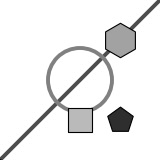
\includegraphics[width=10cm,height=10cm]{slika_1.png}};
\node[below, font=\Large] at (slika1.south) {};

\node[canvas is zy plane at x=0] (slika2) at (-3,0,2) {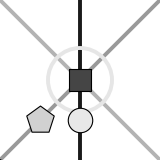
\includegraphics[width=10cm,height=10cm]{slika_2.png}};
\node[below, font=\Large] at (slika2.south) {};

\node[canvas is zy plane at x=0] (slika3) at (-3,0,3) {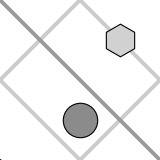
\includegraphics[width=10cm,height=10cm]{slika_3.png}};
\node[below, font=\Large] at (slika3.south) {};

\node[canvas is zy plane at x=0] (slika5) at (-3,0,0) {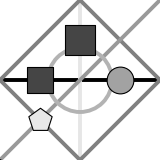
\includegraphics[width=10cm,height=10cm]{slika_5.png}};
\node[below, font=\Large] at (slika5.south) {};

\node[canvas is zy plane at x=0] (slika6) at (-3,0,0) {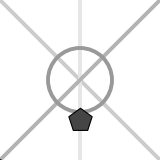
\includegraphics[width=10cm,height=10cm]{slika_6.png}};
\node[below, font=\Large] at (slika6.south) {};

\node[canvas is zy plane at x=0] (slika7) at (-3,0,0) {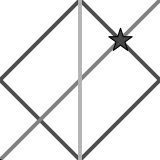
\includegraphics[width=10cm,height=10cm]{slika_7.png}};
\node[below, font=\Large] at (slika7.south) {};

\node[canvas is zy plane at x=0] (slika8) at (-3,0,0) {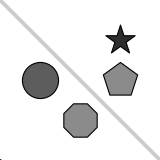
\includegraphics[width=10cm,height=10cm]{slika_8.png}};
\node[below, font=\Large] at (slika8.south) {};

\node[canvas is zy plane at x=0] (slika9) at (-3,0,0) {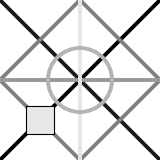
\includegraphics[width=10cm,height=10cm]{slika_9.png}};
\node[below, font=\Large] at (slika9.south) {};

\node[canvas is zy plane at x=0] (slika10) at (-3,0,0) {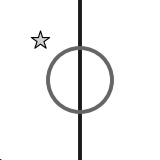
\includegraphics[width=10cm,height=10cm]{slika_10.png}};
\node[below, font=\Large] at (slika10.south) {};

\node[canvas is zy plane at x=0] (slika11) at (-3,0,0) {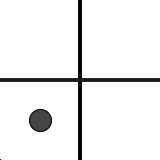
\includegraphics[width=10cm,height=10cm]{slika_11.png}};
\node[below, font=\Large] at (slika11.south) {};

\node[canvas is zy plane at x=0] (slika12) at (-3,0,0) {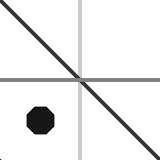
\includegraphics[width=10cm,height=10cm]{slika_12.png}};
\node[below, font=\Large] at (slika12.south) {};

\node[canvas is zy plane at x=0] (slika13) at (-3,0,0) {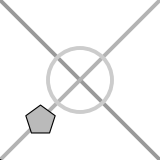
\includegraphics[width=10cm,height=10cm]{slika_13.png}};
\node[below, font=\Large] at (slika13.south) {};

\node[canvas is zy plane at x=0] (slika14) at (-3,0,0) {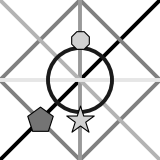
\includegraphics[width=10cm,height=10cm]{slika_14.png}};
\node[below, font=\Large] at (slika14.south) {16 naslaganih panela};

\pic[shift={(2,0,0)}] at (0,0,0) 
    {Box={
        name=conv1,
        caption=,
        xlabel={{16, }},
        zlabel=79,
        fill=\ConvColor,
        height=19,
        width=4,
        depth=19
        }
    };

\pic[shift={(0,0,0)}] at (conv1-east) 
    {Box={
        name=norm1,
        caption=,
        fill=\BatchNorm,
        height=19,
        width=3,
        depth=19
        }
    };

\pic[shift={(0,0,0)}] at (norm1-east) 
    {Box={
        name=relu1,
        caption=,
        fill=\Relu,
        height=19,
        width=3,
        depth=19
        }
    };

\draw [connection]  (-2, 0, 0)    -- node {\midarrow} (conv1-west);

\pic[shift={(2,0,0)}] at (relu1-east) 
    {Box={
        name=conv2,
        caption=,
        xlabel={{16, }},
        zlabel=38,
        fill=\ConvColor,
        height=10,
        width=4,
        depth=10
        }
    };

\pic[shift={(0,0,0)}] at (conv2-east) 
    {Box={
        name=norm2,
        caption=,
        fill=\BatchNorm,
        height=10,
        width=3,
        depth=10
        }
    };

\pic[shift={(0,0,0)}] at (norm2-east) 
    {Box={
        name=relu2,
        caption=,
        fill=\Relu,
        height=10,
        width=3,
        depth=10
        }
    };

\draw [connection]  (relu1-east)    -- node {\midarrow} (conv2-west);

\pic[shift={(2,0,0)}] at (relu2-east) 
    {Box={
        name=conv3,
        caption=,
        xlabel={{16, }},
        zlabel=18,
        fill=\ConvColor,
        height=5,
        width=4,
        depth=5
        }
    };

\pic[shift={(0,0,0)}] at (conv3-east) 
    {Box={
        name=norm3,
        caption=,
        fill=\BatchNorm,
        height=5,
        width=3,
        depth=5
        }
    };

\pic[shift={(0,0,0)}] at (norm3-east) 
    {Box={
        name=relu3,
        caption=,
        fill=\Relu,
        height=5,
        width=3,
        depth=5
        }
    };

\draw [connection]  (relu2-east)    -- node {\midarrow} (conv3-west);

\pic[shift={(2,0,0)}] at (relu3-east) 
    {Box={
        name=conv4,
        caption=,
        xlabel={{16, }},
        zlabel=9,
        fill=\ConvColor,
        height=2,
        width=4,
        depth=2
        }
    };

\pic[shift={(0,0,0)}] at (conv4-east) 
    {Box={
        name=norm4,
        caption=,
        fill=\BatchNorm,
        height=2,
        width=3,
        depth=2
        }
    };

\pic[shift={(0,0,0)}] at (norm4-east) 
    {Box={
        name=relu4,
        caption=,
        fill=\Relu,
        height=2,
        width=3,
        depth=2
        }
    };

\draw [connection]  (relu3-east)    -- node {\midarrow} (conv4-west);

\pic[shift={(2,0,0)}] at (relu4-east) 
    {Box={
        name=linear1,
        caption=,
        zlabel=512,
        fill=\FcColor,
        height=25,
        width=3,
        depth=3
        }
    };

\draw [connection]  (relu4-east)    -- node {\midarrow} (linear1-west);

\pic[shift={(0,0,0)}] at (linear1-east) 
    {Box={
        name=linear2,
        caption=,
        fill=\Relu,
        height=25,
        width=3,
        depth=3
        }
    };

\pic[shift={(0,0,0)}] at (linear2-east) 
    {Box={
        name=Dropout,
        caption=\\,
        fill=\DropoutColor,
        height=25,
        width=3,
        depth=3
        }
    };

\pic[shift={(2,0,0)}] at (Dropout-east) 
    {Box={
        name=linear3,
        caption=,
        zlabel=8,
        fill=\FcColor,
        height=5,
        width=3,
        depth=3
        }
    };

\draw [connection]  (Dropout-east)    -- node {\midarrow} (linear3-west);

\fill[white] (23,8) rectangle ++(-12,-4);
\draw (23,8) rectangle ++(-12,-4);

\filldraw[fill=\ConvColor] (12,7) ++(-0.5,0) circle (0.2);
\node[font=\Large, anchor=west] at (12,7) {\textcolor{black}{Konvolucija (3x3)}};

\filldraw[fill=\BatchNorm] (12,6) ++(-0.5,0) circle (0.2);
\node[font=\Large, anchor=west] at (12,6) {\textcolor{black}{Normalizacija Grupe}};

\filldraw[fill=\Relu] (12,5) ++(-0.5,0) circle (0.2);
\node[font=\Large, anchor=west] at (12,5) {\textcolor{black}{ReLu funkcja}};

\filldraw[fill=\FcColor] (18,7) ++(-0.5,0) circle (0.2);
\node[font=\Large, anchor=west] at (18,7) {\textcolor{black}{Linearni sloj}};

\filldraw[fill=\DropoutColor] (18,6) ++(-0.5,0) circle (0.2);
\node[font=\Large, anchor=west] at (18,6) {\textcolor{black}{Izostavljanje(0.5)}};
    
\end{tikzpicture}
\end{document}
